% ================================
% Landon Buell
% Kevin Short
% Physics 799%
% 30 July 2020 
% ================================


\documentclass[12pt,letterpaper]{article}
\usepackage{amsmath}
\usepackage{amssymb}
\usepackage{float}
\usepackage{caption}
\usepackage{subcaption}
\usepackage{graphicx}
\usepackage{xcolor}
\usepackage[top=2.5cm,left=2.5cm,right=2.5cm]{geometry}


\begin{document}

% ================================================================

\section{The Neural Network}
\label{sec-TheNeuralNetwork}

% ================================================================

\subsection{An Introduction to Neural Networks}
\label{sec-NerualNetworkIntro}

\paragraph*{}The task of algorithmically matching sound files to musical instrument classes in exceedingly difficult through conventional computer programming techniques. Because of the complexity of sound waves, brain's interpretation them, the challenge arises as to how to build some sort of program that could function at a level above general procedural or explicit instructional rules. Rather than \textit{hard-coding} a set of conditions or parameters for a classification program, we seek an architecture that allows for a computer to \textit{learn} and change and update itself as it is presented with more data. Such an algorithm exists in the form of a \textit{Neural Network} \cite{Geron2,Goodfellow,Levine}.

\paragraph*{}A neural network is a mathematical function that seeks to produce an approximation $F^*$, of some usually unknown function $F$ . For audio recognition, $F$ is some function, or series of functions, that occurs in the brain which allows for a listener to take the sensation of audio, and map it to a known musical instrument. For a neural network, a model must construct an approximate function $F^*$ using a set of parameters $\Theta$, which allows the model to map a series of inputs, $x$ (called \textit{features}) to a series of outputs, $y$ (called \textit{predictions}) \cite{Goodfellow,James,Virtanen}.

\paragraph*{}Former YouTube video classification team lead, and current machine learning consultant, Aurelien Geron writes about the relationship between biological brains and mathematical neural networks \cite{Geron}: 
\begin{quote}
Birds inspired us to fly, burdock plants inspired velcro and nature has inspired many other inventions. It seems only logical, then, to look to the brain's architecture for inspiration on how to build an intelligent machine.
\end{quote}
The result of such an analogy is a computer program that is reminiscent of the brain. 

\paragraph*{}Over the course of their lives, humans will learn to map sounds to sources almost effortlessly. Given an example, and the appropriate label, humans can do this with very reasonable accuracy over a wide array of sounds \cite{Olsen,White}. We can simplify the idea of humans recognizing sound as some function or operation that occurs within the brain, accepting an input sound, and produces an output label. Similarly, a neural network can be constructed, presented with \textit{features} of multiple, labeled sound waves and learns a set of parameters $\Theta$ that allows for the mapping to a source.

\paragraph*{}For this particular project, a neural network has been constructed to perform a \textit{classification} task. A classification task involves mapping the input data, $x$ to one of $k$ possible \textit{classes}, each represented by an integer, $0$ through $k-1$. Each of the $k$ classes represents a particular musical instrument that could have produced the sound-wave in the audio file. 

% ================================================================

\newpage

\subsection{The Structure of a Neural Network}
\label{sec-NetworkStructre}

\paragraph*{}A Neural Network is simply a model of a mathematical function, composed of several smaller mathematical functions called \textit{layers} \cite{Goodfellow,Loy}. Each layer represents an operation that takes some real input, typically an array of real double-precision floating-point numbers, and returns a modified array of new double-precision floating-point numbers. The exact nature of this operation can be very different depending on the layer type or where it sits within the network. It is this process of transforming inputs successively in a particular order until an output is attained \cite{Geron,Loy}. This output encodes the models final "decision" given a unique input.

\paragraph*{}Other than inspiration from the brain, Neural Networks are name \textit{networks} because of their nested composition nature. The model can be represented by a linear or acyclic computational graph which successively maps exactly how the repeated composition is structured. In a \textit{feed-forward network}, information is passes successively in one direction. For example functions could be chained together such as \cite{Goodfellow}
\begin{equation}
\label{eqn-FunctionChain}
F(x) = f^{(L-1)}\big[f^{(L-2)}\big[...f^{(1)}\big[f^{(0)}\big[x]\big]\big]...\big]\big]
\end{equation}
Where each function $f^{(l)}$ represents a layer of the network model. The number of layers in a neural network is referred to as the network \textit{depth}. The dimensionality of each layer is referred to as the network \textit{width} \cite{Geron,Loy}.

\paragraph*{}A network model that contains $L$ unique layers is said to be an $L$-Layer Neural Network, with each layer usually indexed by a superscipt, $0$ through $L-1$. Layer $0$ is said to be the \textit{input layer} and layer $L-1$ is said to be the \textit{output layer}. The function that represents a layer $(l)$ is given by 
\begin{equation}
\label{eqn-LayerFunction}
f^{(l)} : x \in \mathbb{R} \rightarrow y \in \mathbb{R}
\end{equation}
The value of $x$ can also be index by layer, we call the array $x^{(l)}$ the \textit{activations} of layer $l$ \cite{Goodfellow,Loy}. 

\paragraph*{}The model is recursive by nature, the activations from one layer, $l-1$, are used to directly produce the activations of the next successive layer $l$. Thus eqn. (\ref{eqn-LayerFunction}) can be alternatively written as:
\begin{equation}
\label{eqn-altLayerFunction}
f^{(l)} : x^{(l-1)} \in \mathbb{R} \rightarrow x^{(l)} \in \mathbb{R}
\end{equation}
The array of activations, $x^{(0)}$, is the raw input given the neural network, most commonly called \textit{features}. Conversely, the activations $x^{(L-1)}$ are commonly called the network \textit{output} \cite{Geron,James,Loy}.



% ================================================================

\newpage

\subsection{Layers Used in Classification Neural Network}
\label{sec-Layers}

\paragraph*{}As stated previously, a neural network is composed of a series of functions that are called successively to transform features (an input) into a prediction (an output). As shown in eqn. (\ref{eqn-altLayerFunction}), each function feeds directly into the next as to form a sort of computational graph \cite{Goodfellow}. 

\paragraph*{}Typically, a layer function can be divided into two portions: (i.) a Linear transformation, with a bias addition, and (ii.) an element-wise activation transformation. This activation function typically is a non-linear function which allows for the modeling of increasingly complex decision-boundaries. Step (i.) is usually in the form of a matrix-vector equation:
\begin{equation}
\label{eqn-matVectEqn}
z^{(l)} = W^{(l)} x^{(l-1)} + b^{(l)}
\end{equation}
Where $W^{(l)}$ is the \textit{weighting-matrix} for layer $l$, $b^{(l)}$ is the \textit{bias-vector} for layer $l$, $z^{(l)}$ are the \textit{linear-activations} for layer $l$ and $x^{(l-1)}$ is the final activations for layer $l-1$.
Step (ii.) is usually given by some \textit{activation function}:
\begin{equation}
\label{eqn-elementActivation}
x^{(l)} = \sigma^{(l)} \big[ z^{(l)} \big]
\end{equation}
Where $x^{(l)}$ is the final activations for layer $l$ and $z^{(l)}$ is given in equation (\ref{eqn-matVectEqn}). $\sigma^{(l)}$ is some activation function, which is often use to enable the modeling of more complex-decision boundaries. 

\paragraph*{}The combination of eqn. (\ref{eqn-matVectEqn}) and eqn. (\ref{eqn-elementActivation}), for a layer $l$ , make up the function represented by that layer, as in eqn. (\ref{eqn-altLayerFunction}). Below, we discuss and describe the types of layer functions that are used to produce the classification model in this project.

% ================

\subsubsection{Dense Layer}

\paragraph*{}The Linear Dense Layer, often just called a \textit{Dense} Layer, or \textit{Fully-Connected} layer for short, was one of the earliest function types used in artificial neural network models \cite{Geron2,Loy}. They are among the most commonly used layer types. A dense layer is composed of a layer of \textit{artifical neurons}, each of which holds a numerical value within it, called the \textit{activation} of that neuron. This idea was developed back from McCulloch and Pitts' work \cite{McCulloch}, and was expanded upon by Frank Rosenblatt in  1957 \cite{Geron}.

\paragraph*{}We model a layer of neurons as a vector of floating-point numbers. Typically, it is required that the array be one-dimensional. Suppose a layer $(l)$ contains $n$ artificial neurons. We denote the array that hold those activations as $x^{(l)}$ and is given by:
\begin{equation}
\label{layer-DenseNeurons}
\vec{x}^{(l)} = \Big[ x_0, x_1, x_2, \hdots , x_{n-2}, x_{n-1} \Big]^T
\end{equation}
The activation of each entry is given by a linear-combination of activations from the previous layer, as outlined in eqn.(\ref{eqn-matVectEqn}) and eqn.(\ref{eqn-elementActivation}).

\paragraph*{}Suppose the layer $l-1$ contains $m$ neurons. Then the weighting-matrix, $W^{(l)}$ has shape $m \times n$, the bias-vector $b^{(l)}$ has shape $m \times 1$. We can denote the function in a similar manner to eqn.(\ref{eqn-altLayerFunction}) as:
\begin{equation}
\label{eqn-FunctionDense}
f^{(l)} : x^{(l-1)} \in \mathbb{R}^{(m \times 1)} \rightarrow x^{(l)} \in \mathbb{R}^{(n \times 1)}
\end{equation}

Thus for a dense layer $l$, the exact values of each activation is given by \cite{Geron,Loy}:
\begin{equation}
\begin{bmatrix}
x_0 \\ x_1 \\ \vdots \\ x_{n-1}
\end{bmatrix}^{(l)} =
\sigma^{(l)} \Bigg(
\begin{bmatrix}
w_{0,0} & w_{0,1} & \hdots & w_{0,m-1} \\
w_{1,0} & w_{1,1} & \hdots & w_{1,m-1} \\
\vdots & \vdots & \ddots & \vdots  \\
w_{n-1,0} & w_{n-1,1} & \hdots & w_{n-1,m-1} 
\end{bmatrix}^{(l)} 
\begin{bmatrix}
x_0 \\ x_1 \\ \vdots \\ x_{m-1}
\end{bmatrix}^{(l-1)} +
\begin{bmatrix}
b_0 \\ b_1 \\ \vdots \\ b_{n-1}
\end{bmatrix}^{(l)} \Bigg)
\end{equation}
or more compactly:
\begin{equation}
\label{eqn-DenseFeedForward}
x^{(l)} = \sigma^{(l)} \Big( W^{(l)} x^{(l-1)} + b^{(l)} \Big)
\end{equation}
Eqn. (\ref{eqn-DenseFeedForward}) is generally referred to as the \textit{dense layer feed-forward equation} \cite{Goodfellow}. 

% ================

\subsubsection{2-Dimensional Convolution Layer}

\paragraph*{}Convolution layers emerged from studying the brain's visual cortex, and have been used from image recognition related tasks for around 40 years. \cite{Geron,Loy}). This layer get's it's name from it's implementation of the mathematical \textit{convolution} function. The 2D discrete-convolution of function $A(i,j)$ and $B(i,j)$ is given by \cite{Goodfellow}:
\begin{equation}
\label{eqn-convolution}
C(i,j) = (A * B)(i,j) = \sum_{u}\sum_{v} A(i,j)B(i - u,j - v)
\end{equation}
Note that convolution is commutative: $(A * B) = (B * A)$. We implement a convolutional layer $f^{(l)})$, by creating a series of $K$ weighting matrices, called \textit{filters}, each of size $m \times n$, where $m,n \in \mathbb{Z}$. Often we choose $m = n$ and call the shape the \textit{convolution kernel size} \cite{Loy, Goodfellow}.

\paragraph*{}In the case of a 2D input array, $x^{(l-1)} \in \mathbb{R}^{(N \times M)}$, the convolutions filters "step" through the input data and repeatedly compute the element-wise product of each $m \times n$ weighting kernel, and the local activation of the $x^{(l-1)}$ array. The step size in each of the 2-dimension is known as the \textit{stride}. Each of the $K$ filters is used to generate a $m \times n$ feature map from the input activation. For an appropriately trained network, some filters may be dedicated to detecting vertical lines, horizontal lines, sharp edges, areas of mostly one color, etc. \cite{Loy,Geron}.

\paragraph*{}In general, for an $N \times M$ input, with kernel size $m \times n$, with stride size $1 \times 1$, and $K$ feature maps.
\begin{equation}
f^{(l)} : x^{(l-1)} \in \mathbb{R}^{(N \times M)} \rightarrow
x^{(l)} \in \mathbb{R}^{([N-n+1] \times [M-m+1] \times K)}
\end{equation}
As an example, consider a single filter map over input $x \in \mathbb{R}^{(4 \times 3)}$ and filter map $W \in \mathbb{R}^{(2 \times 2)}$ as shown in fig. (\ref{fig-2DConvExample}):
\begin{figure}[H]
\label{fig-2DConvExample}
\begin{center}
\begin{subfigure}{0.45\textwidth}
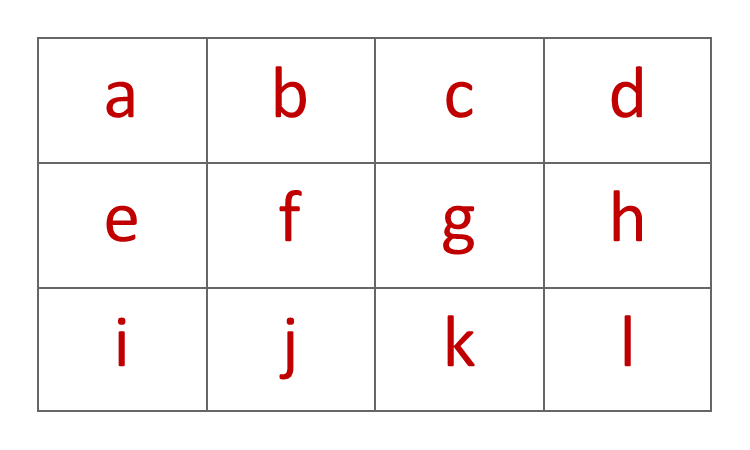
\includegraphics[scale=0.6]{../figures/2DConvExample(a)}
\caption{Input Activations}
\end{subfigure}
\begin{subfigure}{0.45\textwidth}
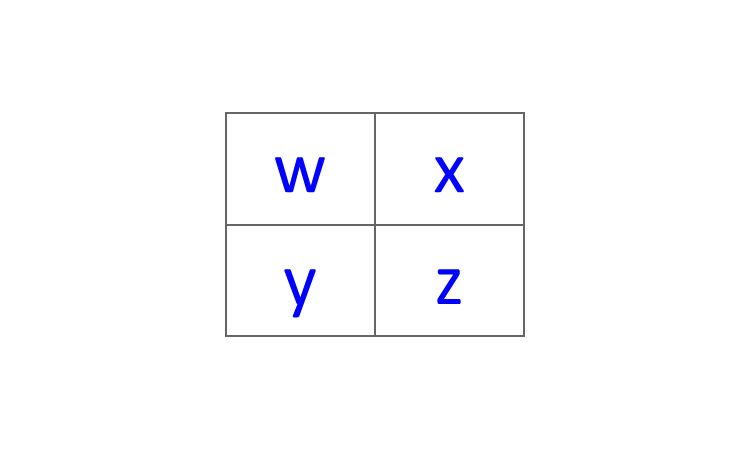
\includegraphics[scale=0.6]{../figures/2DConvExample(b)}
\caption{Convolution Filter}
\end{subfigure}
\begin{subfigure}{0.9\textwidth}
\centering
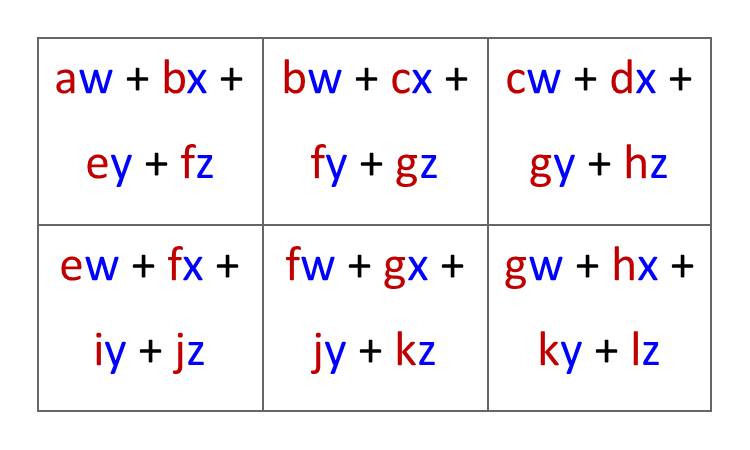
\includegraphics[scale=0.6]{../figures/2DConvExample(c)}
\caption{Convolution Result}
\end{subfigure}
\end{center}
\caption{The result of convolving an input (a) with an filter map (b) is a new set of activations (c). This Image was adapted from Goodfellow, pg. 325 \cite{Goodfellow}}
\end{figure}
Note that formal implementations include a bias vector and an activation function.

\paragraph*{}For 2D convolution over input $x^{(l-1)}$ with feature map $W^{(l)}_k$, producing activations $x^{(l)}$, we compute the activations $x^{(l)}_{k}$ as \cite{Goodfellow}
\begin{equation}
\label{eqn-ConvFeedForward}
x^{(l)}_k = \sigma^{(l)}\bigg[ \Big( \sum_{u=0}^{m-1} \sum_{v=0}^{n-1} x^{(l-1)}(i,j) W^{(l)}_k(i - u,j - v) \Big) + b^{(l)}_k \bigg]
\end{equation}
\textcolor{red}{Please check my math here!}
This operation repeats for each of the $K$ feature maps. Each maps has it's own $n \times m$ weighting matrix and appropriately shaped bias .

\paragraph*{}The convolution layers allows for several advantages. Among these are (i) \textit{sparse-connectivity}: not every single activation (pixel) is connect to every single output pixel, so it is more computationally efficient, (ii) \textit{positional invariance}: key features can be identified regardless of where they are in the layer



% ================

\subsubsection{2-Dimensional Maximum Pooling Layer}

\paragraph*{}A Maximum Pooling layers simply returns the maximum neuron activation in a group of neurons. In the case of 2D Max Pooling, we choose a kernel size to be $m \times n$, just like in the 2D Convolution layer, and extract the maximum value in each window, and then step along accrdoing to the chosen stride size \cite{Loy,Goodfellow}.As an example, consider again figure (\ref{fig-2DConvExample}). Using the $2 \times 2$ kernel on the $3 \times 4$ input, each box would then contain the maximum value of the input activations. We detail this in fig. (\ref{fig-2DMaxPool}):
\begin{figure}[h]
\label{fig-2DMaxPool}
\begin{center}
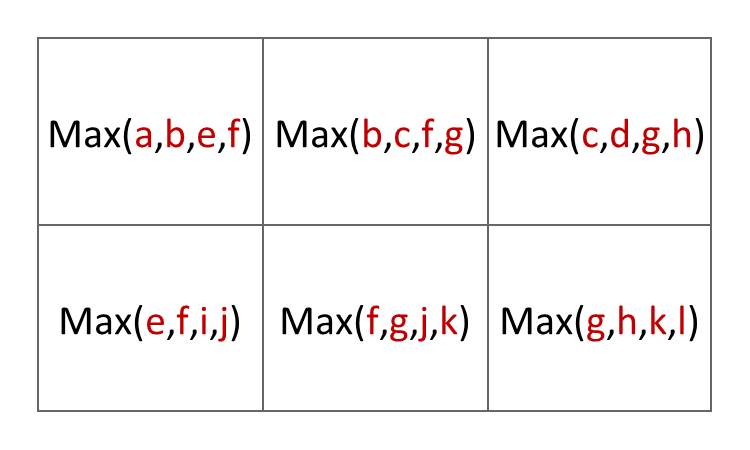
\includegraphics[scale=0.6]{../figures/2DConvExample(d)}
\end{center}
\caption{The result of 2D maximum-pooling an input array. This image was adapted from Loy, pg. 126 \cite{Loy}}
\end{figure} 

\paragraph*{}Pooling layers, such as maximum pooling, average pooling, or similar are typically placed after a layer or a set of layers of convolution. The purpose of this arrangement is to reduce the number of weights, thereby dropping the complexity of the model and ensuring only features with large activation values are preserved \cite{Geron,Loy,Goodfellow}.

% ================

\subsubsection{1-Dimensional Flattening Layer}

\paragraph*{}A flattening layer is used to compress an array with two or more dimensions down into a single dimension. For a flattening layer $l$, multidimensional activations in layer $l-1$ are compressed down into a single dimensional array. We can use function notation to express this as:
\begin{equation}
\label{eqn-FlattenFunction}
f^{(l)} : x^{(l-1)} \in \mathbb{R}^{(M \times N \times ....)} \rightarrow
x^{(l)} \in \mathbb{R}^{(MN...\times 1)}
\end{equation}
The numerical value of each activation is left unchanged. For a layer with activation shape$N \times M$, the resulting activations are reshaped into $NM \times 1$ as shown in eqn (\ref{eqn-FlattenFunction}).

\paragraph*{}Flattening Layer are most commonly used to prepare activations for entry into dense layer or series of dense layers. For example, 2D or 3D images are typically processed with 2D convolution, which may output a 2D or 3D array of activations. Those values are then flattened to 1 dimensions, which can then be passed into dense layers for further processing.

% ================

\subsubsection{1-Dimensional Concatenation Layer}

% ================================================================

\subsection{Activation Functions Used in Network Layers}
\label{sec-ActivationFunctions}

\paragraph*{}Activation functions are a key parameter in the behavior of neural networks. As discussed in sec. (\ref{sec-Training}) a layer function, $f^{(l)}$ is generally composed of a linear transformation, as in eqn. (\ref{eqn-matVectEqn}), and then an element-wise activation function as in eqn. (\ref{eqn-elementActivation}). It is this second step that allows for neural networks to model the incredibly complex decision boundaries that are found in real-world problems \cite{Geron,Loy}. In this section, we detail the activation functions used in out classification neural network. 

\subsubsection{Rectified Linear Unit}



\subsubsection{Softmax}


% ================================================================

\newpage

\subsection{Training a Neural Network}
\label{sec-Training}

\paragraph*{}A neural network's job is to produce an approximation of some function $F$, which we call $F^*$. The model must have a procedure for updating the parameters in $\Theta$ to allow for a reasonable approximation of $F$. To better understand this, we turn to Tom Mitchell's explanation of a learning algorithm \cite{Goodfellow,Mitchell}:
\begin{quote}
A computer program is said to learn from experience $E$ with respect to some class of tasks $T$ and performance measure $P$, if it's performance at tasks in $T$, as measured by $P$, improves with experience $E$.
\end{quote}
Without any human intervention, a model must update itself to improve it's performance at a give task a new information is presented to it. To do this, the model must be constructed with a training procedure in mind. 

\paragraph*{}We consider the set of parameters $\Theta$ as a concatenation of each applicable layer's weighting matrix and bias vector such that:
\begin{equation}
\label{eqn-Theta}
\theta = \big\{
W^{(0)}, b^{(0)}, W^{(1)}, b^{(1)}, W^{(2)}, b^{(2)}, ... ,W^{(L-2)}, b^{(L-2)},W^{(L)}, b^{(L-1)},
\big\}
\end{equation}
We can consider each parameter as just float-point number, which is stored in a weight matrix $W^{(l)}$ or bias vector $b^{(l)}$. Each value for each parameter contributes to the output of the function. In increasingly complicated neural networks, there can be upwards of hundreds of thousands,or even millions of elements in $\theta$ making a neural network a functions that exist is a very high dimensional parameter-space.

\subsubsection{The Cost Function}

\paragraph*{}Suppose we pass a training sample $x^{0})$, with expected outcome $y$, into the neural network . For a perfectly accurate model, we expect the network's final layer, the output layer, $x^{(L-1)}$ to have activations such that $x^{(L-1)} \approx y$. Since the starting parameters of a network are often randomly generated, the prediction for training sample $x^(0)}$ is not likely to be similar to $y$ at all. We introduce a \textit{Cost Function} into our model that compares the difference between the neural output $x^{(L-1)}$ (also called $y^*$) and the desired, or expected output $y$ \cite{Goodfellow,James}.

\paragraph*{}There are various types of cost functions 

\subsubsection{The Optimizer}

% ================================================================

\newpage

\subsection{Chosen Model Architecture}

\paragraph*{}The success of a neural network algorithm is enormously dependent of the strength of the chosen features, rather than the quantity of available data \cite{Geron,Kahn,Liu}. We have derived an appropriate set of inputs arrays \textit{[See Section on Features]}, and constructed a neural network architecture to compliment these features.

\paragraph*{}The full classification neural network used for this project consists of two distinct entry points. This means that rather than presenting the network with one set of input data, $X$, we present the network with two different arrays, $X_1$ and $X_2$. Both arrays are a produce of the same audio file sound wave, and thus share a common training label. Each of the two entry points feed into their own, non-related set of layer functions. The second-to-last layer, the outputs from both neural networks are concatenated into a single dense layer, which is then passed into the output layer, which contains $k$ neurons, one of reach unique class \cite{Loy,Geron}. A visual representation of this architecture can be found in fig. (\ref{fig-NetworkArchitecture}).

\begin{figure}[H]
\label{fig-NetworkArchitecture}
\begin{center}
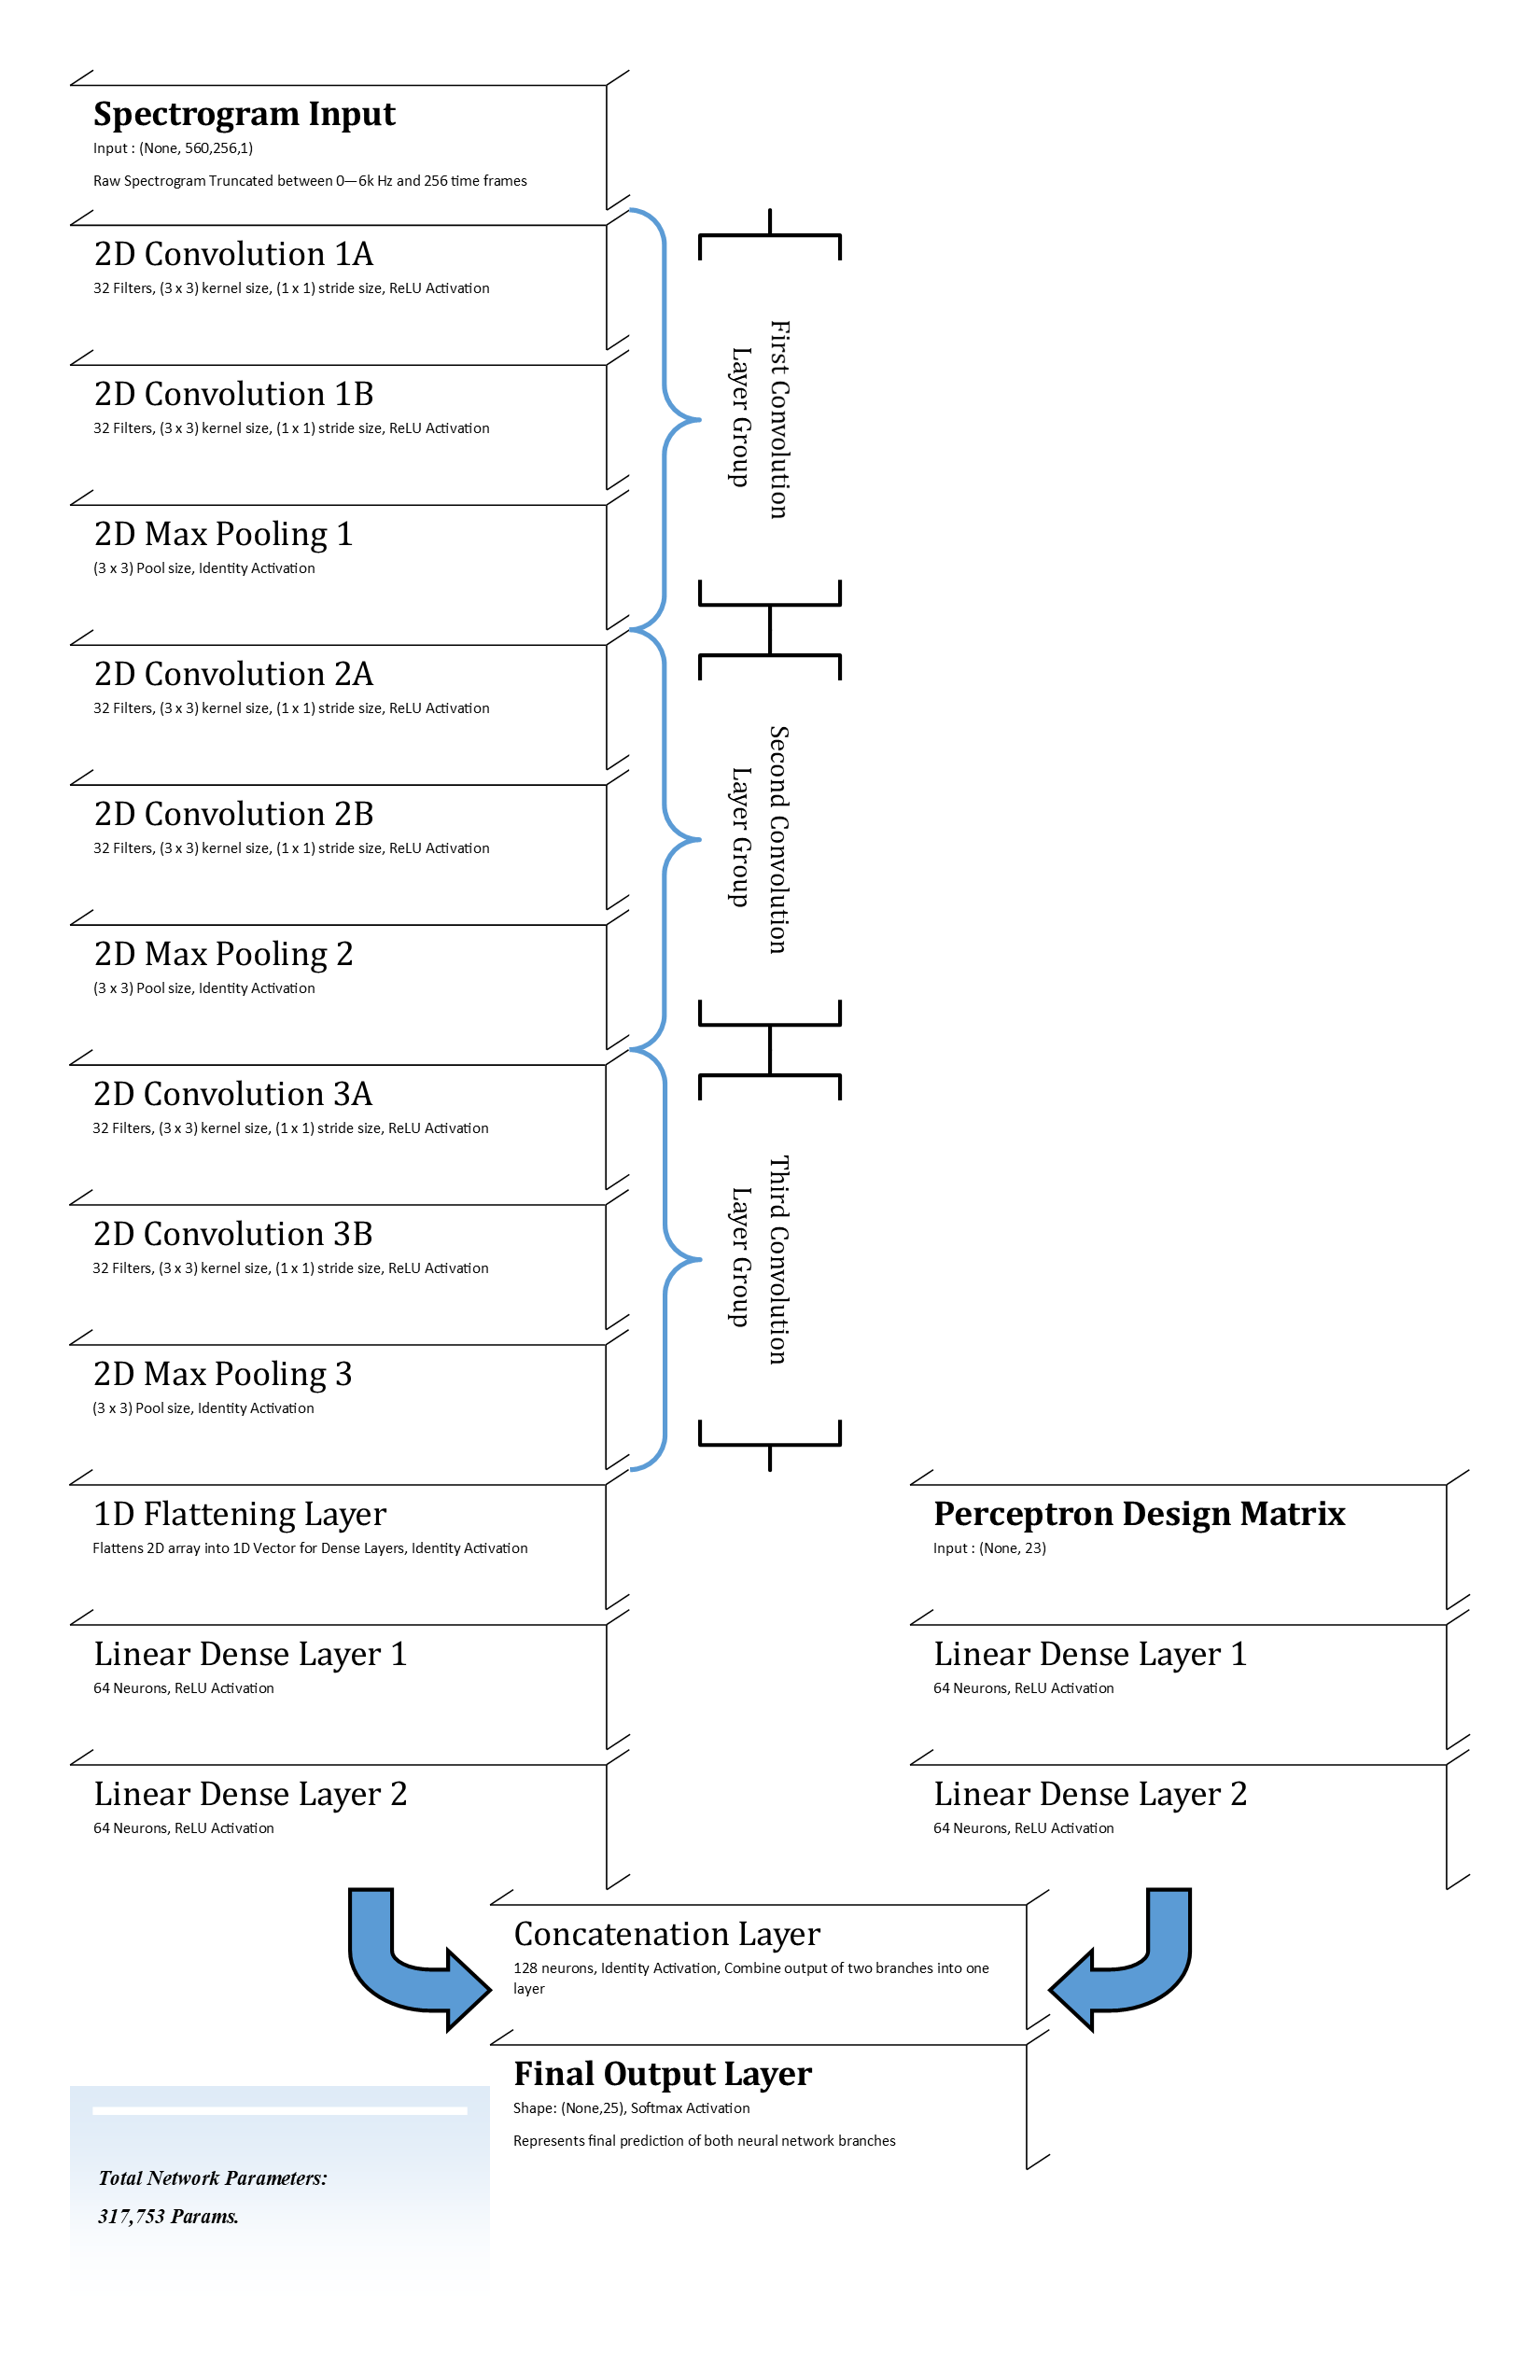
\includegraphics[scale=0.45]{../Figures/NeuralNetworkArchitecture}
\end{center}
\caption{The developed architecture of the audio file classification neural network. The Left branch process an image-like input, the right branch processes a vector-like input. The activations are then merged, and then a single output is produced}
\end{figure}

% ================

\subsubsection{The Spectrogram Branch}

\paragraph*{}The spectrogram branch is pictured on the right side of fig. (\ref{fig-NetworkArchitecture}). A spectrogram is a representation of a sound wave, or signal by representing energy distributions as a function of \textit{time} and \textit{frequency} \cite{White,Olsen,Kahn}. \textcolor{blue}{Details on the creating of the spectrogram can be found in the \textit{features} section of this document.}

\paragraph*{}The input layer of the spectrogram accepts a 4-Dimensional array. The axes, in order of indexing, represents (i) the size of the \textit{mini-batch} of samples, (ii) the pixel width of each sample, (iii) the pixel height of each sample, and (iv) the number of channels in each sample. As a model hyper-parameter, we have chosen each batch to contain $64$ samples. We have also chosen to truncate time and frequency axes (ii \& iii) to contain $560$ frequency bins, and $256$ time-frames. Each image also contains a single channel, which make it gray-scale when visualized. We can denote the 4D shape of the input object into this branch as:
\begin{equation}
\label{eqn-shapeX1}
X_1 \in \mathbb{R}^{(64 \times 560 \times 256 \times 1)}
\end{equation}
Any other shape will be rejected by the model, and an error is raised.

\paragraph*{}After the input layer assert the appropriate shape, the array $X_1$, which is a collection of $64$ spectrograms, is passed into the first of three \textit{Convolution Layer Groups}. These layer groups are inspired from the \textit{VGG-16 Neural Network} architecture \textcolor{red}{[citation needed]}. Each convolution layer group in composed of three individual layers: 
\begin{enumerate}
\item A 2-Dimensional Convolution layer, using $32$ filters, a $3 \times 3$ kernel, a $1 \times 1$ step size, and a ReLU activation function,
\item A 2-Dimensional Convolution layer, using $32$ filters, a $3 \times 3$ kernel, a $1 \times 1$ step size, and a ReLU activation function,
\item A 2-Dimensional Maximum Pooling layer using a $3 \times 3$ pooling size, and an Identity activation function
\end{enumerate}  
The Convolution layers convoluted over the middle two axes of the data (over space and time in the spectrogram). 

\paragraph*{}By grouping layers in this structure, each of the $32$ filters passes over a $3 \times 3$ area, and then again. The result is 

% ================

\subsubsection{The Perceptron Branch}

\paragraph*{} The Perceptron branch is picture on the right side of fig. (\ref{fig-NetworkArchitecture}), notice that it is considerably smaller in side and complexity than it's neighbor. Rather than accept an image-like input, the perception simply takes a vector-like input of properties of a larger data set - in this case, each waveform. We call these properties \textit{features} \cite{Geron,Kahn,Virtanen}. \textcolor{blue}{Details on the creating of these features can be found in the \textit{features} section of this document.}

\paragraph*{}The input layer of the perceptron accepts a 2-Dimensional array. The axes, in order of indexing, represent (i) the size of the \textit{mini-batch} of samples, (ii) the number of features for each sample. We use the same model hyper-paramater of $64$ samples per batch, and have developed $23$ unique clssification features that have been derived from time-space and frequency-space representations of the audio file data. We can denote the 2D shape if the input object into this branch as:
\begin{equation}
\label{eqn-shapeX2}
X_2 \in \mathbb{R}^{(64 \times 20)}
\end{equation}
Again, any other shape will be rejected by the model, and an error is raised.

% ================

\subsubsection{The Final Output Branch}

\paragraph*{}


% ================================================================










% ================================================================

\newpage

\begin{thebibliography}{9}
\bibliographystyle{apalike}

\bibitem{Geron}
Geron, Aurelien. \textit{Hands-on Machine Learning with Scikit-Learn and TensorFlow: Concepts, Tools, and Techniques to Build Intelligent Systems}. O'Reilly, 2017.

\bibitem{Geron2}
Geron, Aurelien. \textit{Hands-on Machine Learning with Scikit-Learn and TensorFlow: Concepts, Tools, and Techniques to Build Intelligent Systems}. 2nd ed., O'Reilly, 2019.

\bibitem{Goodfellow}
Goodfellow, Ian, et al.\textit{Deep Learning}. MIT Press, 2017.

\bibitem{James}
James, Gareth, et al. \textit{An Introduction to Statistical Learning with Applications in R}. Springer, 2017.

\bibitem{Kahn}
Khan, M. Kashif Saeed, and Wasfi G. Al-Khatib. “Machine-Learning Based Classification of Speech and Music.” Multimedia Systems, vol. 12, no. 1, 2006, pp. 55–67., doi:10.1007/s00530-006-0034-0.

\bibitem{Levine}
Levine, Daniel S. \textit{Introduction to Neural and Cognitive Modeling}. 3rd ed., Routledge, 2019.

\bibitem{Liu}
Liu, Zhu, et al. "Audio Feature Extraction and Analysis for Scene Segmentation and Classification." Journal of VLSI Signal Processing, vol. 20, 1998, pp. 61–79.

\bibitem{Loy}
Loy, James , \textit{Neural Network Projects with Python}. Packt Publishing, 2019

\bibitem{McCulloch}
McCulloch, Warren S., and Walter Pitts. "A Logical Calculus of the Ideas Immanent in Nervous Activity." \textit{The Bulletin of Mathematical Biophysics}, vol. 5, no. 4, 1943, pp. 115–133.

\bibitem{Mierswa}
Mierswa, Ingo, and Katharina Morik. "Automatic Feature Extraction for Classifying Audio Data." \textit{Machine Learning}, vol. 58, no. 2-3, 2005, pp. 127–149., doi:10.1007/s10994-005-5824-7.

\bibitem{Mitchell}
Mitchell, Tom Michael. Machine Learning. 1st ed., McGraw-Hill, 1997.

\bibitem{Olsen}
Olson, Harry E. \textit{Music, Physics and Engineering}. 2nd ed., Dover Publications, 1967.

\bibitem{Peatross}
Peatross, Justin, and Michael Ware. \textit{Physics of Light and Optics.} Brigham Young University, Department of Physics, 2015.

\bibitem{Petrik}
Petrik, Marek. "Introduction to Deep Learning." Machine Learning. 20 April. 2020, Durham, New Hampshire.

\bibitem{Short}
Short, K. and Garcia R.A. 2006. "Signal Analysis Using the Complex Spectral Phase Evolution (CSPE) Method." AES: \textit{Audio Engineering Society Convention Paper}.

\bibitem{Virtanen}
Virtanen, Tuomas, et al. \textit{Computational Analysis of Sound Scenes and Events.} Springer, 2018.

\bibitem{White}
White, Harvey Elliott, and Donald H. White. \textit{Physics and Music: the Science of Musical Sound}. Dover Publications, Inc., 2019.

\bibitem{Zhang}
Zhang, Tong, and C.-C. Jay Kuo. “Content-Based Classification and Retrieval of Audio.” \textit{Advanced Signal Processing Algorithms, Architectures, and Implementations VIII}, 2 Oct. 1998, pp. 432–443., doi:10.1117/12.325703.

\end{thebibliography}

% ================================================================

\end{document}
